\section{Politik}
Inden for caching findes der politiker, der definere hvor i cachen, ting skal gemmes.
Der findes \textit{Placeringspolitik} og \textit{Erstatnignspolitik}.
\textbf{Placeringspolitik} definerer hvor i cachen at en blok placeres, hvor \textbf{Erstatningspolitik} definerer, hvad der skal erstattes.
\section{Hit og miss}
Hit og miss forekommer, når der laves en forespørgsel til cachen.
Et hit eksisterer, når der laves en forespørgsel til cachen, og den efterspurgte værdi findes i cachen.
Et miss er modsat, når der laves en forespørgsel, og den efterspurgte værdi ikke eksisterer i cachen, hvorved den skal hentes i hukommelsen.
\subsection{Kold miss}
Et koldt miss, også kaldet et tvungent miss, opstår når cachen er tom. Dette betyder at der ikke er nogen værdier i cachen, og der derfor kun kan forekomme et miss.
\subsection{Konflikt miss}
Et konflikt forekommer når flere blokke spørger efter den samme plads, men cachen stadig har flere pladser tilgængelig.
Dog har de fleste cache implementationer restriktioner, der er sat for at undgå denne type miss.
Dette kan eksempelvis være at blok \verb|B| skal placeres i \verb|B mod 4| på niveau k.
\subsection{Kapacitets miss}
Dette forekommer når mængden af aktive caceh blokke (working sets) overgår cachens kapacitet.
\section{Typer af cache}
Der findes følgende typer af caching i hukommelses-hierakiet.
\begin{table}[h!]
    \centering
    \begin{tabular}{lllll}
        \hline
        Cache type&Hvad caches&Hvor er cachen&Cycler&Styret af\\\hline
        Registre&4-8 bytes&CPU kerne&0&Compiler\\
        TLB&Addresse overs.&On-chip TLB&0&Hardware MMU\\
        L1 cache&64-byte blokke&On-chip L1&4&Hardware\\
        L2 cache&64-byte blokke&On-chip L2&10&Hardware\\
        Virtuel hukommelse&4-KB sider&Primær huk.&100&Hardware + OS\\
        Buffer cache&Dele af filer&Primær huk.&100&OS\\
        Disk cache&Disk sektor&Disk controller&100000&Disk firmware\\
        Netværks buffer cache&Dele af filer&Lokal disk&10000000&NFSC\\
        Browser cache&Websider&Lokal disk&10000000&Webbrowser\\
        Webcache&Websider&Servers&1000000000&Proxy server\\\hline
    \end{tabular}
    \caption{Caching i hukommelses-hierakiet}
    \label{tab:memhier}
\end{table}

\section{Cache opbygning}
Cachen er opbygget af blokke, af størrelsen $S\cdot E$ elementer. 
En blok ser ud som vist i \cref{fig:cacheblk}
\begin{figure}[h!]
    \centering
    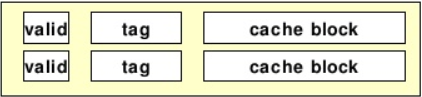
\includegraphics[width=\textwidth]{figures/block.png}
    \caption{Repræsentation af en cache blok}
    \label{fig:cacheblk}
\end{figure}
En sådan blok består af en \textit{Valid} bit, der fortæller om blokken indeholder information, der kan bruges i den givne kontekst.
Der findes også et antal bytes, der gemmer på den ønskede information.
Yderligere indeholder den et markat \textit{tag}, der bruges til at skældne mellem information i cache-linjen, fra hvor det starter i hukommelsen.

For hurtigt at kunne fremsøge information i cachen, opdeles addressen for det ord der ledes efter.
Denne deles i \textit{tag}, \textit{index} og \textit{offset}.
De mindst betydende bits, bruges som offset, de midterste bits bruges til sæt indeks, og de mest betydende bits, bruges til tagget.
For sæt indeks, gælder det at $2^s=S$, altså mængden af sæt i cachen.
Offset vil for et 8-byte ord altid være 3, da offset er 0-indekseret, og derfor ikke må overskride antal gyldige bytes.
Jvf. \cref{tab:bits}.
Dette skyldes at man vil kunne addressere alle bytes i blokken.
De resterende bits, bruges til at danne et tag, for at kunne skældne mellem sæt.

For at kunne tjekke sæt, tag og værdi, kan den givne addresse konverteres til binære tal, hvorved det binære tal kan opdeles i de respektive grupper.
For et 2-byte ord \verb|0xAC| (\verb|1001 1011|), i en cache med 8 sæt, betyder det at strukturen vil se ud som vist i \cref{tab:2byteword}.
\begin{table}[h!]
    \centering
    \begin{tabular}{|c|c|c|c|c|c|c|c|}
        \hline
        7&6&5&4&3&2&1&0\\\hline
        t&t&s&s&s&b&b&b\\\hline
    \end{tabular}
    \caption{Opdeling af 2-byte ord}
    \label{tab:2byteword}
\end{table}
Med denne tabel i tankerne, kan ordet nu opdeles som \verb|10.01 1.011|, hvorved tag, sæt, offset og værdi kan findes.
\textbf{Bemærk} at offset er 0-indekseret.
\section{Lokalitet}
Om lokalitet kan følgende siges.
\begin{itemize}
    \item Programmer der ofte tilgår de samme variabler har god temporal lokalitet.
    \item Programmer med \textit{Stride-k} reference mønster. 
    Jo mindre \textit{Stride} jo bedre, hvor programmer med et \textit{Stride-1} mønster, har den bedste spatialle lokalitet.
    Dette skyldes at programmet ikke skal hoppe i hukommelsen.
    \item Løkker har god temporal og spatial lokalitet, med respekt til operationerne og stride.
    Des mindre løkke-krop, des bedre lokalitet.
\end{itemize}
\section{Caching}

